% -*- latex -*-
%%%%%%%%%%%%%%%%%%%%%%%%%%%%%%%%%%%%%%%%%%%%%%%%%%%%%%%%%%%%%%%%
%%%%%%%%%%%%%%%%%%%%%%%%%%%%%%%%%%%%%%%%%%%%%%%%%%%%%%%%%%%%%%%%
%%%%
%%%% This text file is part of the source of 
%%%% `Introduction to High-Performance Scientific Computing'
%%%% by Victor Eijkhout, copyright 2012-6
%%%%
%%%% This book is distributed under a Creative Commons Attribution 3.0
%%%% Unported (CC BY 3.0) license and made possible by funding from
%%%% The Saylor Foundation \url{http://www.saylor.org}.
%%%%
%%%%
%%%%%%%%%%%%%%%%%%%%%%%%%%%%%%%%%%%%%%%%%%%%%%%%%%%%%%%%%%%%%%%%
%%%%%%%%%%%%%%%%%%%%%%%%%%%%%%%%%%%%%%%%%%%%%%%%%%%%%%%%%%%%%%%%

\index{N-body problems|(}

In chapter \ref{ch:odepde} we looked at continuous phenomena, such as
the behaviour of a heated rod in the entire interval $[0,1]$ over a
certain time period. There are also applications where you may be
interested in a finite number of points. One such application is the
study of collections of particles, possibly very big particles such as
planets or stars, under the influence of a force such as gravity or
the electrical force. (There can also be external forces, which we
will ignore; also we assume there are no collisions, otherwise we need
to incorporate nearest-neighbour interactions.) This type of problems
is known as N-body problems; for an introduction
see \url{http://www.scholarpedia.org/article/N-body_simulations_(gravitational)}.

\begin{wrapfigure}{r}{2.5in}
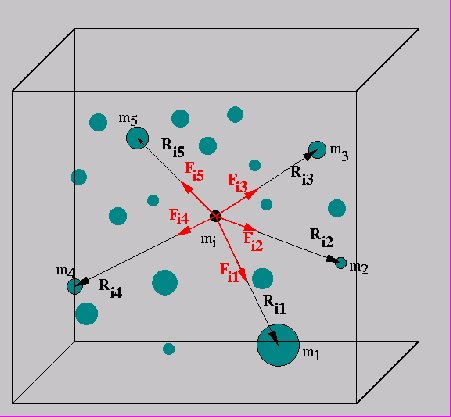
\includegraphics[scale=.4]{nbody_pic}
\caption{Summing all forces on a particle}
\hbox{}\kern-1.5in\hbox{}
\end{wrapfigure}
%
A basic algorithm for this problem is easy enough:
\begin{itemize}
\item choose some small time interval,
\item calculate the forces on each particle, given the locations of
  all the particles,
\item move the position of each particle as if the force on it stays
  constant throughout that interval.
\end{itemize}
For a small enough time interval this algorithm gives a reasonable approximation to the truth. 

The last step, updating the particle positions, is easy and completely
parallel: the problem is in evaluating the forces. In a naive way this
calculation is simple enough, and even completely parallel:

  \begin{tabbing}
    for \=each particle $i$\\
    \>for \= each particle $j$\\
    \>\> let $\bar r_{ij}$ be the vector between $i$ and $j$;\\
    \>\> then the force on $i$ because of $j$ is\\
    \>\> $\quad f_{ij} = -\bar r_{ij}\frac{m_im_j}{|r_{ij}|}$\\
    \>\> (where $m_i,m_j$ are the masses or charges) and\\
    \>\> $f_{ji}=-f_{ij}$.
  \end{tabbing}

The main objection to this algorithm is that it has quadratic computational
complexity: for $N$ particles, the number of operations is~$O(N^2)$.

\begin{exercise}
  If we had $N$ processors, the computations for one update step would
  take time~$O(N)$.  What is the communication complexity? Hint: is
  there a collective operations you can use?
\end{exercise}

Several algorithms have been invented to get the sequential complexity
down to $O(N\log N)$ or even $O(N)$. As might be expected, these are
harder to implement than the naive algorithm. We will discuss a
popular method: the \indexterm{Barnes-Hut algorithm}~\cite{BarnesHut},
which has $O(N\log N)$ complexity.

\Level 0 {The Barnes-Hut algorithm}
\index{Barnes-Hut algorithm|(}

The basic observation that leads to a reduction in complexity is the
following. If you are calculating the forces on two particles
$i_1,i_2$ that are close together, coming from two particles $j_1,j_2$
that are also close together, you can clump $j_1,j_2$ together into
one particle, and use that for both~$i_1,i_2$.

Next, the algorithm uses a recursive division of space, in two
dimensions in quadrants and in three dimensions in octants; see
figure~\ref{fig:bh-quadrants}.
\begin{figure}[ht]
  \hbox{%
  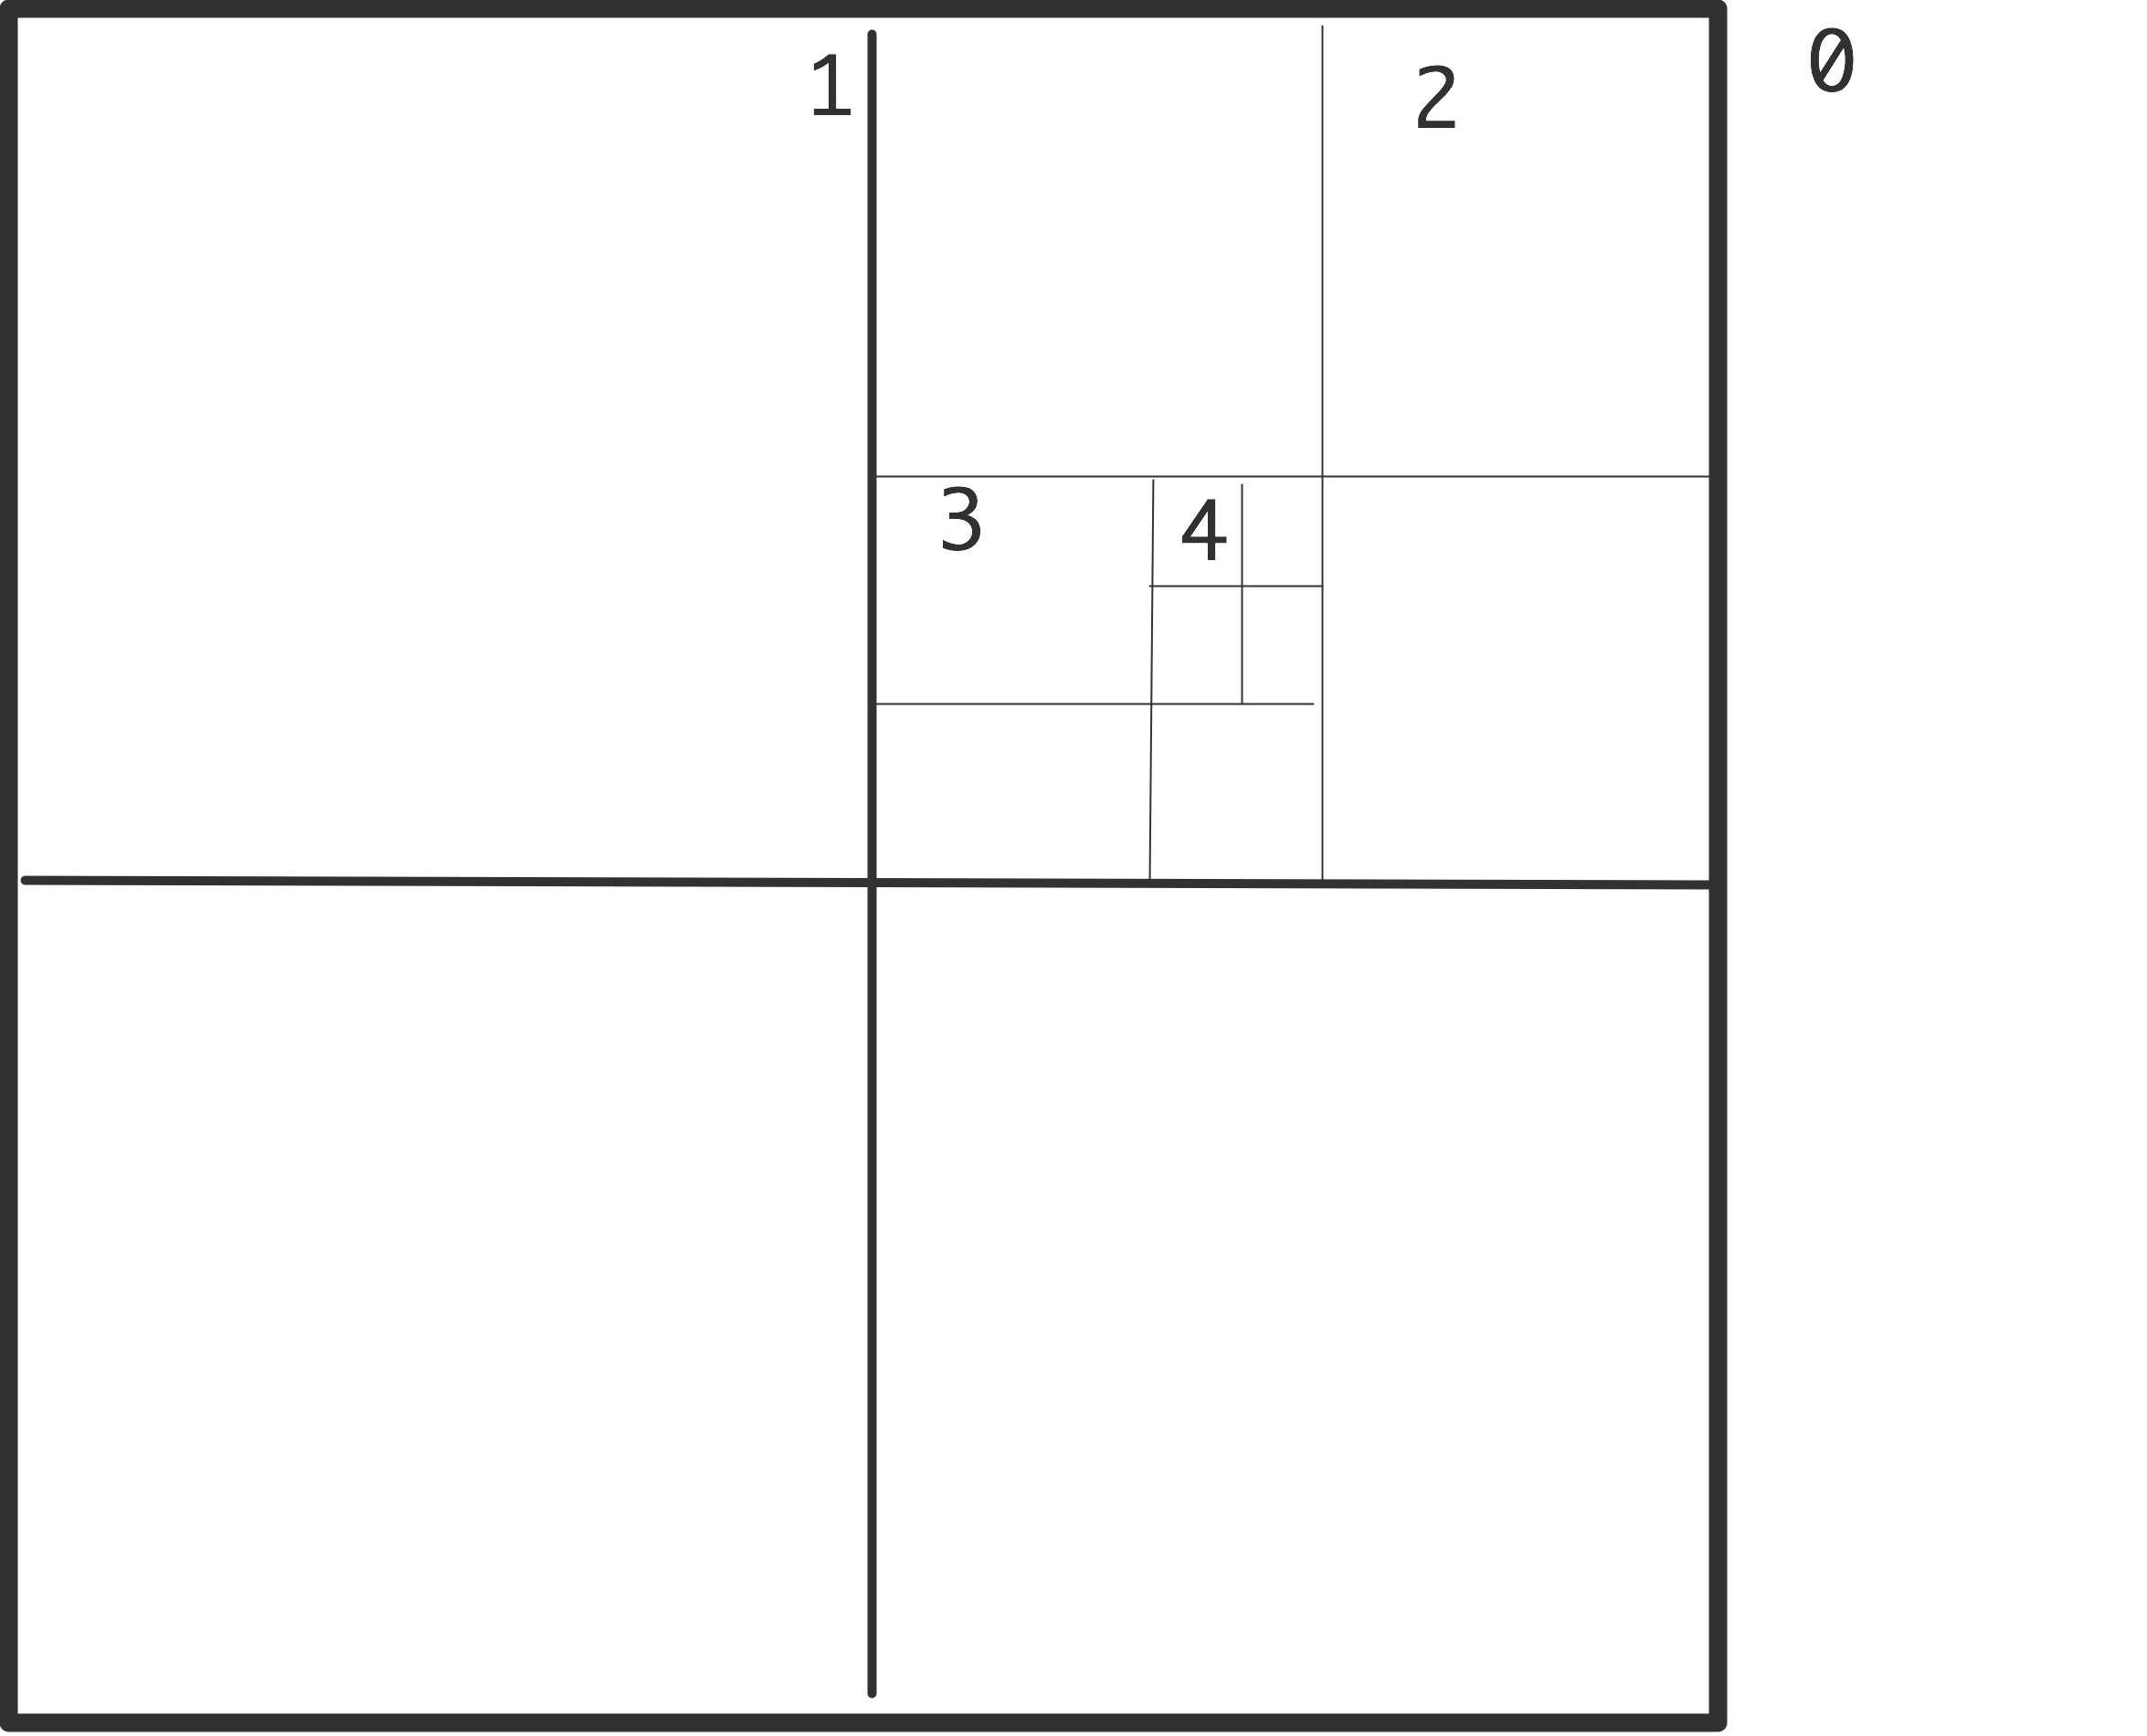
\includegraphics[scale=.1]{graphics/bh-quadrants}
  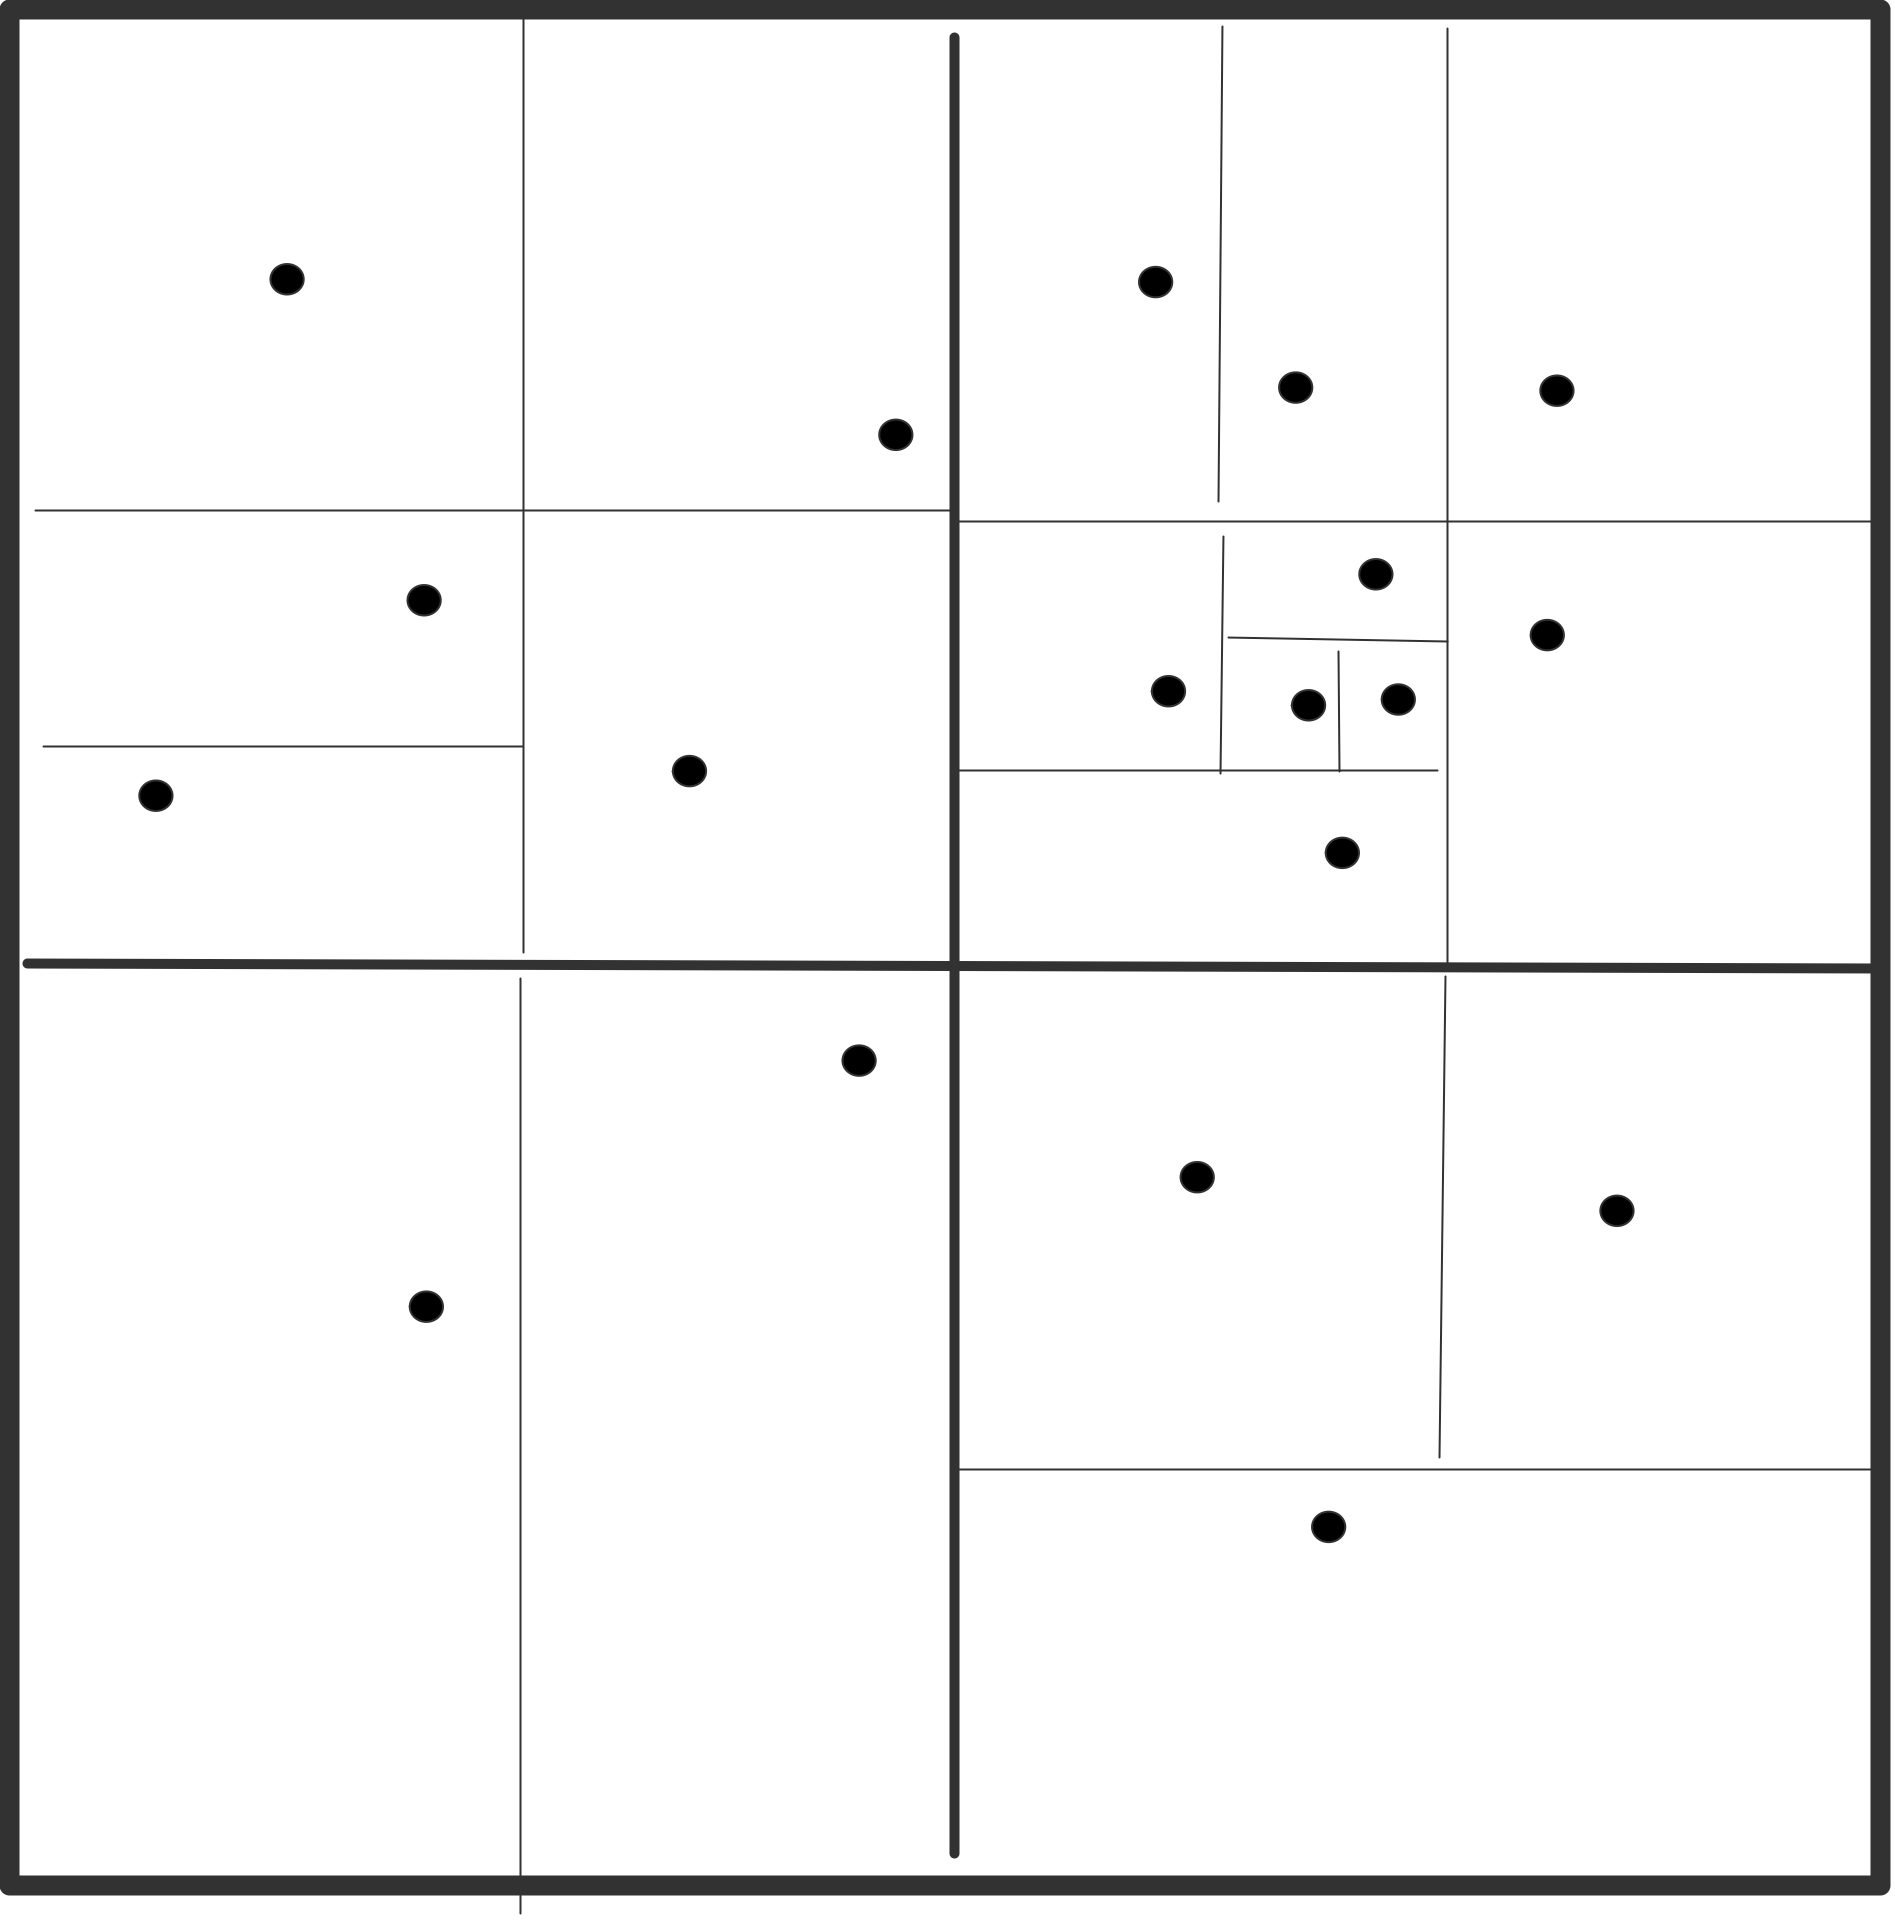
\includegraphics[scale=.1]{graphics/bh-quadrants-filled}%
  }
  \caption{Recursive subdivision of a domain in quadrants with levels
    indicated (left); actual subdivision with one particle per box (right)}
  \label{fig:bh-quadrants}
\end{figure}

The algorithm is then as follows. First total mass and center of mass
are computed for all cells on all levels:
\begin{quotation}
  \begin{tabbing}
    for \=each level $\ell$, from fine to coarse:\\
    \>for \=each cell $c$ on level $\ell$:\\
    \>\> compute \=the total mass and center of mass\\
    \>\>\> for cell $c$ by considering its children\\
    \> if there are no particles in this cell,\\
    \>\> set its mass to zero
  \end{tabbing}
\end{quotation}
Then the levels are used to compute the interaction with each particle:
\begin{quotation}
  \begin{tabbing}
    for \=each particle $p$:\\
    \>for \=each cell $c$ on the top level\\
    \>\>if $c$ \=is far enough away from $p$:\\
    \>\>\>use the total mass and center of mass of $c$;\\
    \>\>otherwise consider the children of $c$
  \end{tabbing}
\end{quotation}

\begin{wrapfigure}{r}{2.5in}
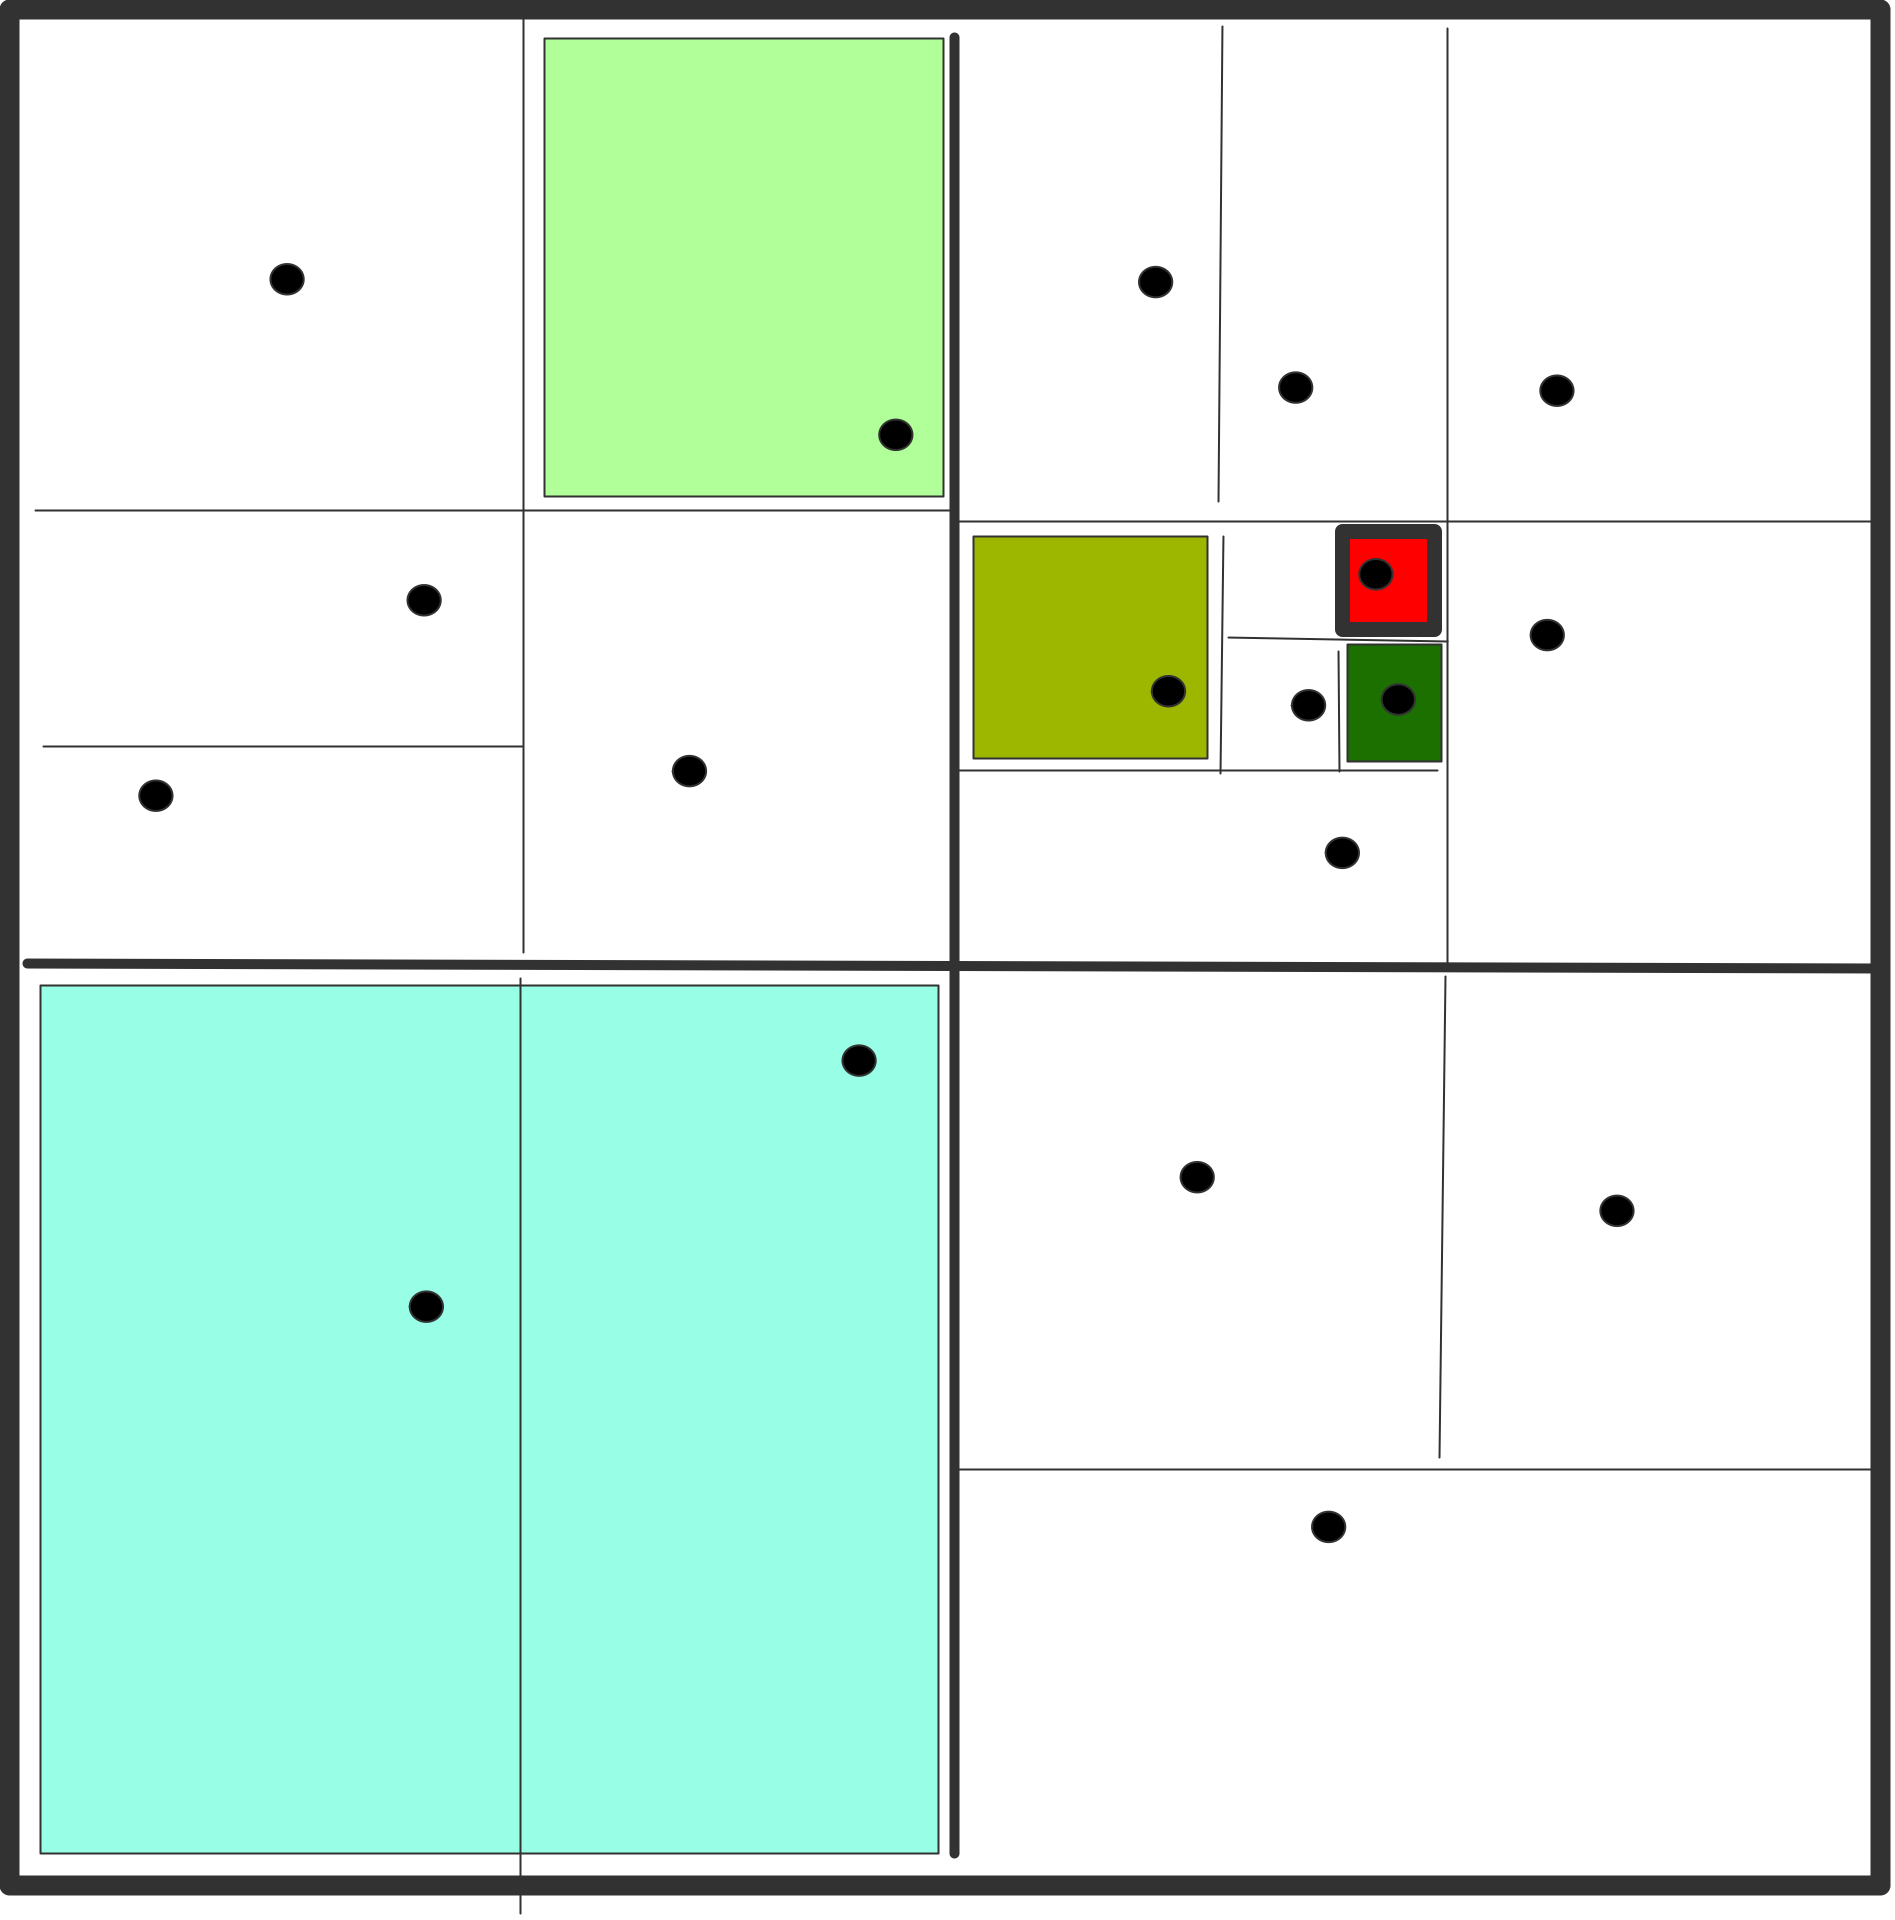
\includegraphics[scale=.08]{bh-quadrants-ratio}
\caption{Boxes with constant distance/diameter ratio}
%\hbox{}\kern-2in\hbox{}
\label{fig:bh-cellratio}
\end{wrapfigure}
%
The test on whether a cell is far enough away is typically implemented
as the ratio of its diameter to its distance being small enough. This
is sometimes referred to as the `cell opening criterium'. In this manner, 
each particle interacts with a number of concentric rings of cells,
each next ring of double width; see figure~\ref{fig:bh-cellratio}.

This algorithm is easy to realize if the cells are
organized in a tree. In the three-dimensional case, each cell has
eight children, so this is known as an \indexterm{octtree}.

The computation of centres of masses has to be done each time after
the particles move. Updating can be less expensive than computing from
scratch. Also, it can happen that a particle crosses a cell border, in
which case the data structure needs to be updated. In the worst case,
a particle moves into a cell that used to be empty.

\index{Barnes-Hut algorithm|)}

\Level 0 {The Fast Multipole Method}

The \indexac{FMM} computes an expression for the potential at every point,
not the force as does Barnes-Hut.  \ac{FMM} uses more information than the
mass and center of the particles in a box. This more complicated
expansion is more accurate, but also more expensive. In compensation,
the FMM uses a fixed set of boxes to compute the potential, rather
than a set varying with the accuracy parameter theta, and location of
the center of mass.

However, computationally the \ac{FMM} is much like the Barnes-Hut
method so we will discuss their implementation jointly.

\Level 0 {Full computation}

Despite the above methods for judicious approximation, there are also
efforts at full calculation of the $N^2$ interactions; see for
instance the \indexterm{NBODY6} code of Sverre Aarseth;
see \url{http://www.ast.cam.ac.uk/~sverre/web/pages/home.htm}.
Such codes use high order integrators and adaptive time steps.
Fast implementation on the \indexterm{Grape computer} exist;
general parallelization is typically hard because of the need
for regular load balancing.

\Level 0 {Implementation}

Octtree methods offer some challenges on high performance
architectures. First of all, the problem is irregular, and secondly,
the irregularity dynamically changes. The second aspect is mostly a
problem in distributed memory, and it
needs \indextermbus{load}{rebalancing}; see section~\ref{sec:load}. In
this section we concentrated on the force calculation in a single
step.

\Level 1 {Vectorization}

The structure of a problem as in figure~\ref{fig:bh-quadrants} is
quite irregular. This is a problem for vectorization on the small
scale of \indexac{SSE}/\indexac{AVX} instructions and on the large
scale of vector pipeline processors (see section~\ref{sec:simd} for an
explanation of both). Program steps `for all children of a certain box
do something' will be of irregular length, and data will possibly be
not stored in a regular manner.

This problem can be alleviated by subdividing the grid even if this
means having empty boxes. If the bottom level is fully divided, there
will always be eight (in three dimension) particles to operate
on. Higher levels can also be filled in, but this means an increasing
number of empty boxes on the lower levels, so there is a trade-off
between increased work and increasing efficiency.

\Level 1 {Shared memory implementation}

Executed on a sequential architecture, this algorithm has complexity
$O(N\log N)$. It is clear that this algorithm will also work on shared
memory if each particle is turned into a task. Since not all cells
contain particles, tasks will have a different running time.

\Level 1 {Distributed memory implementation}

The above shared-memory version of the Barnes-Hut algorithm can not
immediately be used in a distributed memory context, since each
particle can in principle access information from any part of the
total data. It is possible to realize an implementation along these
lines using a \indextermsub{hashed}{octtree}, but we will not persue
this.

We observe data access is more structured than it seems at
first. Consider a particle $p$ and the cells on level~$\ell$ that it
interacts with. Particles located close to $p$ will interact with the
same cells, so we can rearrange interaction by looking at cells on
level~$\ell$ and the other cells on the same level that they interact
with.

This gives us the following algorithm~\cite{Katzenelson:nbody}: the
calculation of centres of mass become a calculation of the force
$g^{(\ell)}_p$ exerted \emph{by} a particle~$p$ on level~$\ell$:
\begin{quotation}
  \begin{tabbing}
    for \=level $\ell$ from one above the finest to the coarsest:\\
    \>for \=each cell $c$ on level $\ell$\\
    \>\>let $g^{(\ell)}_c$ be the \=combination of the $g^{(\ell+1)}_i$
    for all children $i$ of $c$
  \end{tabbing}
\end{quotation}
With this we compute the force \emph{on} a cell:
\begin{quotation}
  \begin{tabbing}
    for \=level $\ell$ from one below the coarses to the finest:\\
    \>for \=each cell $c$ on level $\ell$:\\
    \>\>let $f^{(\ell)}_c$ \=be the sum of\\
    \>\>\>1. the force $f^{(\ell-1)}_p$ on the parent $p$ of $c$, and\\
    \>\>\>2. the sums $g^{(\ell)}_i$ for \=all $i$ on level $\ell$ that\\
    \>\>\>\>satisfy the cell opening criterium
  \end{tabbing}
\end{quotation}

We see that on each level, each cell now only interacts with a small
number of neighbours on that level. In the first half of the algorithm
we go up the tree using only parent-child relations between
cells. Presumably this is fairly easy.

The second half of the algorithm uses more complicated data
access. The cells~$i$ in the second term are all at some distance from
the cell~$c$ on which we are computing the force. In graph terms these
cells can be described as cousins: children of a sibling of $c$'s
parent. If the opening criterium is made sharper, we use second
cousins: grandchildren of the sibling of $c$'s grandparent, et cetera.


\begin{exercise}
  Argue that this force calculation operation has much in common,
  structurally, with the sparse matrix-vector product.
\end{exercise}

In the shared memory case we already remarked that different subtrees
take different time to process, but, since we are likely to have more
tasks than processor cores, this will all even out. With distributed
memory we lack the possibility to assign work to arbitrary processors,
so we need to assign load carefully. \acfp{SFC} can be used here 
to good effect (see section~\ref{sec:space-filling}).

\index{N-body problems|)}

\endinput 

http://www.cs.berkeley.edu/~demmel/cs267/lecture27/lecture27.html

Interaction
between discrete elements:
\begin{itemize}
\item external
\item nearby 
\item far
\end{itemize}

External forces are simple and conveniently parallel.

Nearby forces are easy to handle if spatial domain decomposition is
used: at best ghost regions needed.

Load imbalance because of particle migration.

Far-field forces are difficult because every particle interacts with
every other: naive algorithms are $O(n^2)$.

Particle-mesh methods: move particles to nearby mesh points, use the
fact that the far-field equation satisfies a PDE that is easy to
solve, use FFT or multigrid (complexity $O(n\log n)$, calculate forces
by interpolation.

Approximation by letting faraway particles act as group:
\begin{enumerate}
\item Barnes-Hut
\item \acfp{FMM}
\end{enumerate}
Also $n\log n$ complexity.
